% The projective conic V(zy-x^2) meeting the line V(y-z) at two points.
% Source: book/tex/alg-geom/bezout.tex (§ Bezout's theorem).
\documentclass[border=2mm]{standalone}
\usepackage{tikz}\usepackage{amssymb}
\begin{document}
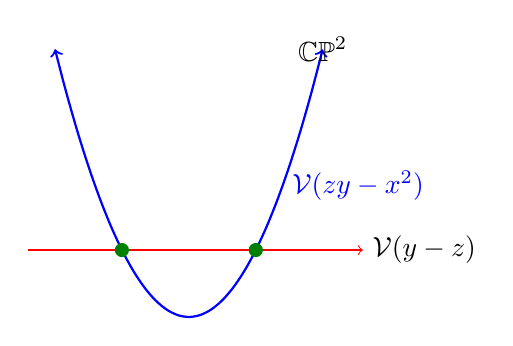
\begin{tikzpicture}[scale=0.85]
  \draw[red,->] (-2.4,0) -- (2.6,0) node[right,black] {$\mathcal V(y-z)$};
  \draw[blue,thick,<->] plot[domain=-2:2,smooth] (\x,{\x*\x-1});
  \node[blue,right] at (1.4,0.96) {$\mathcal V(zy-x^2)$};
  \node at (2,3) {$\mathbb{CP}^2$};
  \fill[green!50!black] (1,0) circle (3pt);
  \fill[green!50!black] (-1,0) circle (3pt);
\end{tikzpicture}
\end{document}
